%*****************************************
\chapter{Short History of mobile computing}\label{ch:history}
%*****************************************

How you define mobile computing plays a huge role in its history, because depending on the definition, it can begin as early as 1971 or as late 1984.

\begin{quotation}
Mobile computing is human-computer interaction by which a computer is expected to be transported during normal usage.\footnote{\url{http://en.wikipedia.org/wiki/Mobile_computing}}
\end{quotation}

If you go with 1971 as the beginning of mobile computing, you come across a very simple calculator that was very advanced for the time. The Busicom LE-120A 'Handy-LE' was the first true pocket sized calculator. Impressive as it may be for the time, a calculator is not something many people would consider as proper computing.

In 1981 the Osborne 1 portable computer came to the market. It was the very first computer designed for users to pack up and carry. The Osborne 1 offered a 5-inch diagonal screen, two full size floppy drives, a keyboard that snapped onto the system, and a handle in the back for easy carrying. But, at 11 kg in weight, it is difficult to consider it as truly portable.\footnote{\url{http://oldcomputers.net/osborne-1.html}}

In 1982 the GRiD Compass 1101 was released. Considered by many to be the grandfather of current laptops, the Compass 1101 was the first portable computer to include the now ubiquitous clamshell design that all modern laptops have, and weighing in at only 4.5 kg, it was the first truly portable computer.\footnote{\url{http://oldcomputers.net/grid1101.html}}

Here is where the story we find interesting begins, but since this thesis caters for a different type of portable computing device, we need to fast forward a little bit in time to 1991 to encounter the first pocket computer, the Psion Series 3.

Since 1982, portable computing devices have become smaller and smarter and in 1991 Psion released the first palmtop minicomputer, a personal organizer that featured a word processor, a spreadsheet, a contacts database, a sketch program, a calculator and a clock.\footnote{\url{http://www.computerworlduk.com/slideshow/mobile-wireless/3267504/}}

But Psion wasn't alone for long. In 1992 Apple Computer released their \ac{PDA} Device called the Newton, but the popularity of these devices was eclipsed when Palm released the Palm Pilot 1000 in 1996. Like every other \ac{PDA} the Pilot let you keep a to do list, a calendar, a contacts database and short memos all in a small, stylus input-based handheld device, but Palm's Graffiti handwriting recognition technology did better job at accepting stylus input than the Newton and earlier handwriting systems did, thus the Pilot became more popular than its competitors.\footnote{\url{http://www.computerworlduk.com/slideshow/mobile-wireless/3267504/}}

After 1996 many different manufactures entered the \ac{PDA} market, and Palm continued to innovate on its line of devices, but in 2002 a cellular phone company called Research in Motion came up with the BlackBerry 5810, a \ac{PDA} that featured phone and email functionality. This device popularized several technologies that users value in smartphones today, such as push email and end-to-end data encryption.\footnote{See above}

Innovations kept being made every year, with different devices coming to market and combining phones with \ac{PDA}s. The first smartphones came around the same time and they too started incorporating more and more features.

By 2007 smartphones were almost omnipresent in the enterprise world, but they were still too expensive and not user friendly enough for the mass market. That is until Apple released the first iPhone, with its intuitive interface and powerful computing ability, it changed the way smartphones were made, removing physical keyboards and making the entire experience as easy and pleasant as possible.

%Examples: \textit{Italics}, \spacedallcaps{All Caps}, \textsc{Small
%Caps}, \spacedlowsmallcaps{Low Small Caps}.

\enlargethispage{2cm}
\begin{figure}[bth]
        \myfloatalign
        \subfloat[Osborne 1]
        {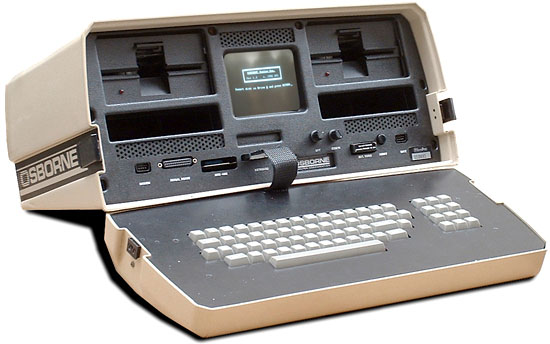
\includegraphics[width=.45\linewidth]{gfx/osborne}} \quad
        \subfloat[GRiD Compass 1101]
        {\label{fig:example-b}%
         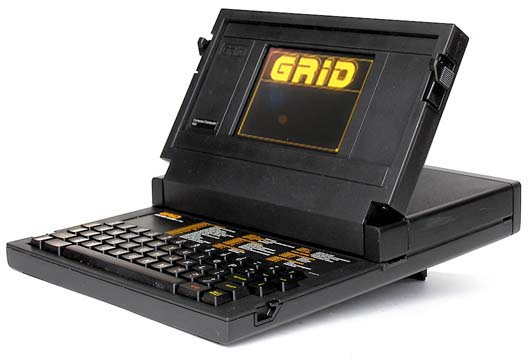
\includegraphics[width=.45\linewidth]{gfx/compass}} \\
        \subfloat[Palm Pilot 1000]
        {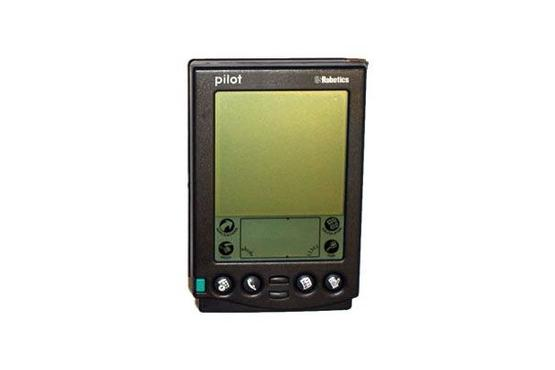
\includegraphics[width=.45\linewidth]{gfx/palm}} \quad
        \subfloat[BlackBerry 5810]
        {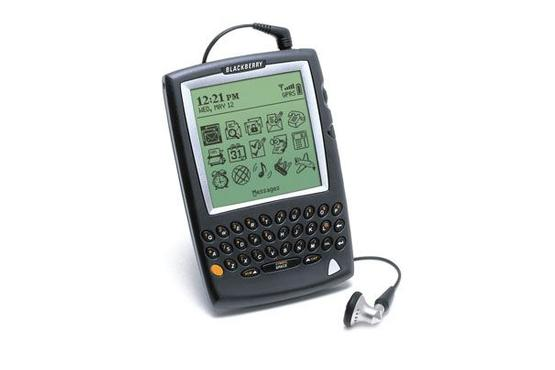
\includegraphics[width=.45\linewidth]{gfx/blackberry}}
        \caption[First mobile computing devices]{First mobile computing devices}\label{fig:example}
\end{figure}